\chapter{Introducere}

\paragraph{}
\^ In zilele noastre, societatea se confrunt\u a tot mai mult cu diverse probleme tehnice \^ in mediul online, industrial, cotidian etc. P\^ an\u a de cur\^ and, aceste probleme puteau fi rezolvate doar cu ajutorul unui specialist \^ in domeniul respectiv. Dup\u a cum \c stim, omul reprezint\u a o resurs\u a limitat\u a c\^ and vine vorba de suport tehnic, deoarece cererile pot fi numeroase, \^ in consecin\c t\u a raspunsul primit poate fi \^ intarziat. De asemenea, trebuie luat in considerare costul prohibitiv de \^ intre\c tinere a unor persoane responsabile cu acest tip de suport.

\paragraph{}
Recent, diverse companii de succes precum Google [1], Facebook[2], Microsoft [3], Apple [4] \c si al\c tii au f\u acut un demers spre adoptarea unor sisteme inteligente de comunica\c tie numite chatbots. \^ In cazul chatbots-ilor orienta\c ti pe suport tehnic, scopul lor este tocmai de a imita sprijinul pe care o persoan\u a real\u a \^ il poate oferi. Un sistem computa\c tional inteligent poate fi folosit pentru a r\u aspunde multor cereri simultane, iar costurile de intre\c tinere sunt mici – practic, odat\u a ce sistemul este dezvoltat, este necesar\u a doar expunerea lui, de exemplu ca serviciu web. Cu c\^ at tehnologia \c si munca de cercetare \^ in aceast\u a arie progreseaz\u a, cu at\^ at sistemele de suport automat devin din ce \^ in ce mai inteligente \c si mai apropiate de ce un om este capabil s\u a ofere [19-21]. Se preconizeaz\u a c\u a \^ in urm\u atorii zece ani, aceste sisteme vor fi capabile s\u a \^ inlocuiasc\u a cu succes o mul\c time de sarcini. Tot a\c sa cum automatizarea industrial\u a de producere a vehiculelor reprezint\u a un standard \^ in era contemporan\u a, a\c sa vor reprezenta \c si ace\c sti asisten\c ti conversa\c tionali un standard \^ in anii ce vor urma.

\paragraph{}
Majoritatea modelelor actuale se bazeaz\u a pe un tip de oferire a unor r\u aspunsuri predefinite. Aceste tipuri de sisteme pot oferi doar solu\c tii existente, nefiind capabile de a genera nimic nou. Pe de alt\u a parte, chatbots-ii baza\c ti pe inteligen\c t\u a artificial\u a reprezint\u a cea mai scalabil\u a modalitate de comunicare \^ intre clien\c ti \c si mediile de afaceri care le sunt dedicate [5].

\paragraph{}
Vorbim deci de evolu\c tia unor modele de chatbots bazate pe pattern matching c\u atre unele bazate pe modele generative, care, precum omul, pot emite r\u aspunsuri bazate pe experien\c te anterioare. \^ In ultimii ani, ramura inteligen\c tei artificiale numit\u a machine learning  (\^ inv\u a\c tare automat\u a) a luat amploare \^ in acest\u a direc\c tie prin curentul numit deep learning [6-8]. Acest curent a produs o mul\c time de rezultate spectaculoase at\^ at \^ in direc\c tia proces\u arii naturale de limbaj c\^ at \c si a proces\u arii de imagini. 

\paragraph{}
Problema asisten\c tilor conversa\c tionali este una de procesare a limbajului natural. Sistemul trebuie s\u a fie capabil s\u a "\^ in\c teleag\u a" informa\c tia primit\u a de la o persoan\u a \c si s\u a produc\u a un raspuns c\^ at mai coerent \c si util. \^ Ins\u a cum \^ in\c telege un calculator o limb\u a? Pentru a r\u aspunde la aceast\u a \^ intrebare, vom face o analogie la cum \^ inva\c t\u a un om o limb\u a. Porne\c ste de la anumite cuvinte de baz\u a iar apoi pe baza acestora, \^ inva\c t\u a cuvinte tot mai complexe. \^ Incepe s\u a creeze fraze prin care leag\u a aceste cuvinte precum \c si gramatica specific\u a limbajului. Practic, totul se bazeaz\u a pe o anumit\u a experien\c t\u a trecut\u a. Conversa\c tia este o modalitate ce faciliteaz\u a \c si impulsioneaz\u a deprinderea limbajului: omul este pus \^ in fa\c ta unor contexte de utilizare, fenomen ce \^ int\u are\c ste deprinderea de utilizare a cuvintelor sau expresiior individuale. Fiecare cuv\^ ant nou \^ inv\u a\c tat reprezint\u a o experien\c t\u a spre \^ inv\u a\c tarea \^ in continuare a limbajului. \^ Inc\u a un lucru la care omul este bun este capabilitatea de a \^ intre\c tine o conversa\c tie lung\u a cu o alt\u a persoan\u a \c si s\u a re\c tin\u a tot felul de informa\c tii noi pe parcurs.

\paragraph{}
\^ In abord\u arile de chatbot actuale se dore\c ste imitarea acestei modalit\u a\c ti de \^ inv\u a\c tare pentru un sistem computa\c tional. Modelarea cea mai puternic\u a \^ in ziua de azi pentru o astfel de problem\u a este oferit\u a de deep learning [6-8]. Folosind un num\u ar mai mare de neuroni fa\c t\u a de arhitecturile shallow folosite p\^ an\u a la \^ inceputul anilor 2000 \c si plec\^ and de la seturi de instruire masive - \^ in cazul de fa\c t\u a corpusuri de text cu c\^ at mai multe fraze \^ in limba pe care o dorim a fi \^ inv\u a\c tat\u a – se formeaz\u a modele generative care pot produce continuarea unor propozi\c tii, fraze etc. Ideea din spatele abord\u arii deep learning este c\u a sistemul devine mai inteligent pe m\u asur\u a ce avem tot mai multe date - \^ in acest caz, spe\c te de conversa\c tii. Pentru a procesa o asemenea cantitate de date de instruire este nevoie de putere computa\c tional\u a pe m\u asur\u a. Asta presupune pe scurt, capacitate hardware. Calculele matematice efectuate pentru \^ inv\u a\c tarea unui limbaj de c\u atre un sistem sunt complexe \c si numeroase (de ordinul sutelor de milioane). Folosirea unui procesor, chiar multicore de ultim\u a genera\c tie, de\c si o idee posibil\u a, este considerat\u a a duce la sugrumarea procesului de instruire. 

\paragraph{}
\^ In locul microprocesorarelor se prefer\u a folosirea de pl\u aci grafice (Graphical Processing Units, GPU). Ini\c tial acestea au fost dezvoltate pentru rulare rapid\u a de jocuri, dar poten\c tialul lor a fost rapid intuit \c si exploatat prin programare paralel\u a. Deoarece placa video con\c tine mult mai multe nuclee de procesare (c\^ ateva mii, comparate cu cele 4-8 nuclee tradi\c tionale dintr-un microprocesor actual), este preferat\u a programarea \c si rularea modelelor computa\c tionale pe GPU. Sunt dezvoltate biblioteci care faciliteaz\u a unui programator dezvoltarea de aplica\c tii de machine learning pe GPU: Tensorflow [9], Theano [10], Caffe [11], Keras [12] etc.

\section{Motiva\c tia alegerii temei}
\paragraph{}
O poten\c tial\u a utilizare este augmentarea sistemului de creare a tichetelor: Universitatea Transilvania folose\c ste \^ in mod curent un sistem de suport tehnic bazat pe tichete, care apoi sunt procesate de persoane reale pentru rezolvare (Figura 1.1, Figura 1.2). Un tichet presupune primirea de la solicitant a c\^ at mai multor detalii legate de problem\u a. De regul\u a, din lips\u a de experien\c t\u a, detaliile furnizate sunt insuficiente pentru o solu\c tionare eficient\u a, motiv pentru care, dup\u a completarea ini\c tial\u a a tichetului se poart\u a un dialog \^ intre suportul IT \c si solicitant pentru aflarea de informa\c tii suplimentare legate de problema raportat\u a. Acest lucru consum\u a timp; se poate \^ imbun\u a\c ti procesul prin demararea c\^ at mai rapid\u a a unui dialog solicitant - chatbot prin care s\u a se completeze tichetul c\^ at mai fidel.

\begin{figure}[H]
\centering
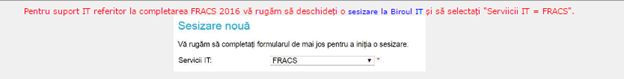
\includegraphics[width=0.8\textwidth]{tichet_unitbv1}
\caption{Sistem pentru suport IT pe portalul Universit\u a\c tii}
\end{figure}

\begin{figure}[H]
\centering
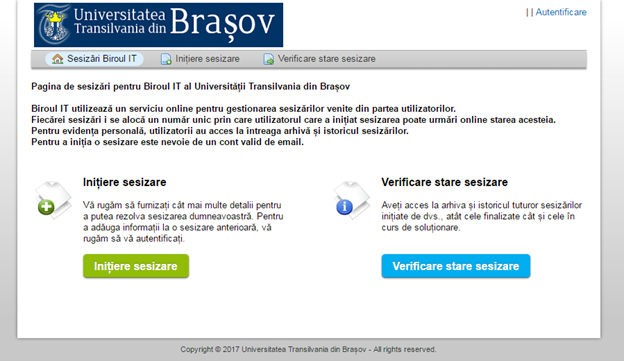
\includegraphics[width=0.8\textwidth]{tichet_unitbv2}
\caption{Pagina de sesiz\u ari pentru biroul IT}
\end{figure}

\paragraph{}
Un sistem artificial de chatbot, pe baza dialogurilor anterioare \^ inregistrate \c si a unei similitudini a cererilor, ar putea fie s\u a solicite mai multe detalii, fie s\u a sugereze pa\c si de rezolvare. \^ In cazul \^ in care exist\u a un corpus de cuno\c stin\c te (knowledge-base) dat de experien\c tele anterioare (dialoguri, solu\c tii date), e posibil ca el s\u a fie exploatat \^ in mod automat [19-21].

\section{Structura lucr\u arii}

\paragraph{}
TODO


\section{Acknowledgement}

\paragraph{}
TODO